\chapter{Title}
\section{More Trajectory Estimation}
\begin{figure}[H]
    \centering
    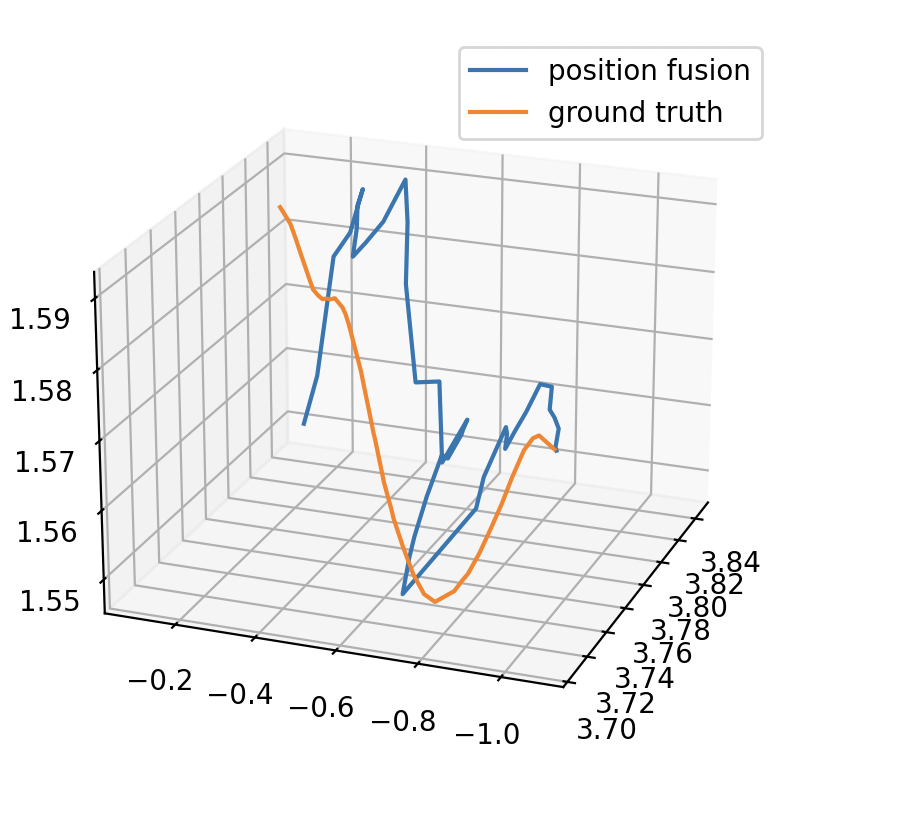
\includegraphics[width=.6\linewidth]{Pictures/sensor_fusion/2425_1s_test.png}
    \caption{Trajectory of Sensor Fusion}
    \label{fig:sensor_fusion_1}
\end{figure}

\begin{figure}[H]
    \centering
    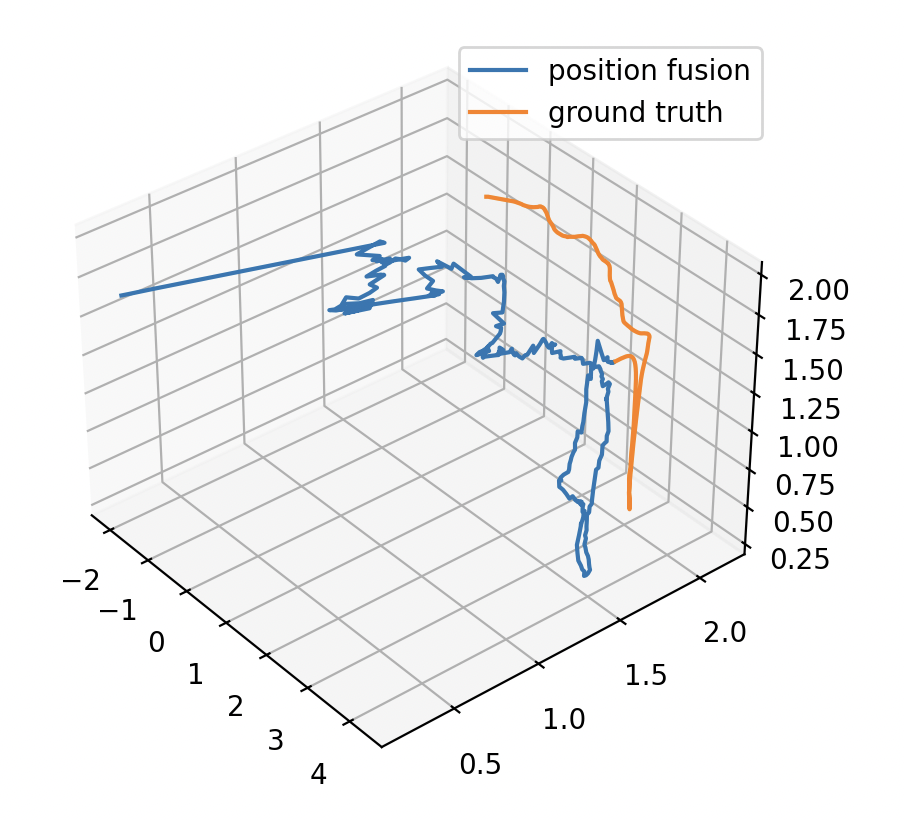
\includegraphics[width=.6\linewidth]{Pictures/sensor_fusion/10s_test.png}
    \caption{Trajectory of Sensor Fusion}
    \label{fig:sensor_fusion_2}
\end{figure}

\clearpage
\section{3D Motion Capture System}
\begin{figure}[H]
    \centering
    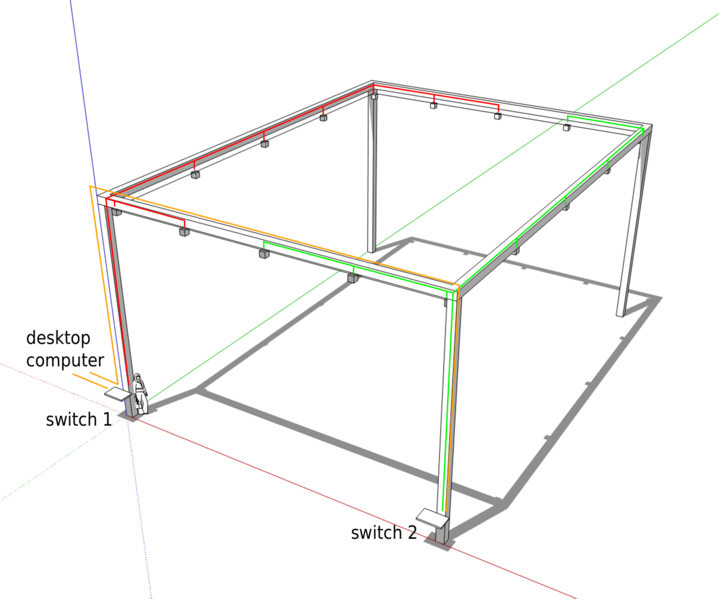
\includegraphics[width=.6\textwidth]{Pictures/settingofdrone/optitrack.png}
    \caption{3D Motion Capture System.}
    \label{fig:optitrack}
\end{figure}
\begin{figure}[H]
    \centering
    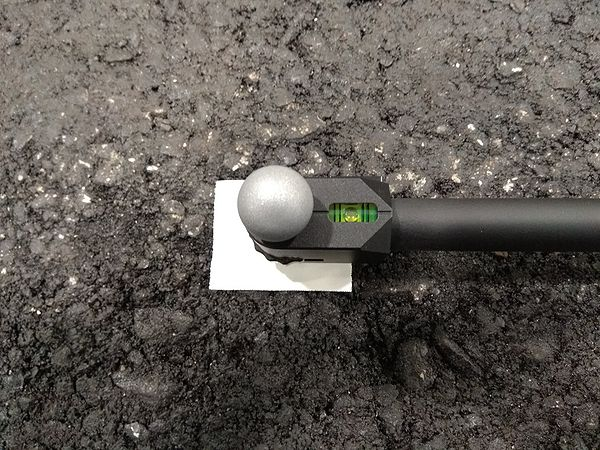
\includegraphics[width=.5\textwidth]{Pictures/settingofdrone/rfball.png}
    \caption{Markers for System Detection.}
    \label{fig:rfball}
\end{figure}
\begin{figure}[H]
    \centering
    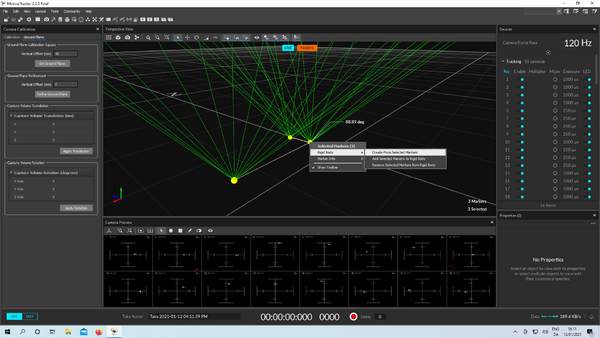
\includegraphics[width=.5\textwidth]{Pictures/settingofdrone/rigidbody.png}\hfill
    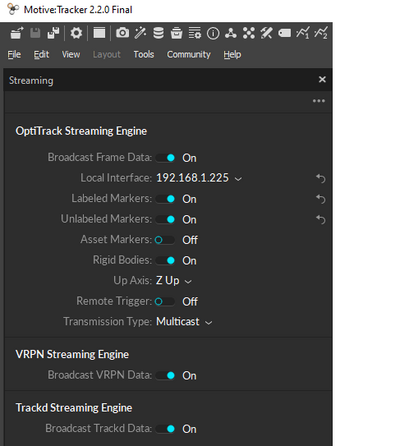
\includegraphics[width=.3\textwidth]{Pictures/settingofdrone/datastreaming.png}
    \caption{Creating Rigid Body and Enabling Steaming}
    \label{fig:steaming}
\end{figure}